\subsection{Propriedades do Conjunto Típico}
\begin{frame}%[allowframebreaks]
  \frametitle{Propriedades do Conjunto Típico}
  \begin{theorem}[Propriedades do Conjunto Típico $A_\epsilon^{(n)}$]
  \begin{enumerate}
  \item Se $(x_1, x_2, \ldots, x_n) \in A_\epsilon^{(n)}$, então
        \begin{equation}
        H(X) - \epsilon \leq - \frac{1}{n} \log p(x_1, x_2, \ldots, x_n) \leq H(X) + \epsilon
        \end{equation}
  \item $p(A_\epsilon^{(n)}) = p\left( \left\{ x: x \in A_\epsilon^{(n)} \right\} \right) > 1 - \epsilon$ para $n$ grande suficiente, para todo $\epsilon > 0$.
  \item Limite superior: $\vert A_\epsilon^{(n)} \vert \leq 2^{n(H(X)+\epsilon)}$, onde $\vert A_\epsilon^{(n)} \vert$ é o número de elementos no conjunto $A_\epsilon^{(n)}$.
  \item Limite inferior: $\vert A_\epsilon^{(n)} \vert \geq (1-\epsilon) 2^{n(H(X) - \epsilon)}$ para $n$ grande suficiente.
  \end{enumerate}
  \end{theorem}

  \begin{itemize}
  \item O conjunto típico possui, essencialmente, probabilidade $1$ (algo típico irá tipicamente ocorrer).
  \item Todos os itens neste conjunto terão a mesma probabilidade $\approx 2^{-nH}$.
  \end{itemize}
\end{frame}

\begin{frame}%[allowframebreaks]
  \frametitle{Exemplo $K=\vert \{0,1\} \vert$: Conjunto Típico}
  \begin{itemize}
  \item Suponha o Ensaio de Bernoulli com distribuição uniforme, $K=2$, 
        $\mathcal{X} = \{0,1\}$, $p=0.5$, entropia $H=1$ e
        $\vert A_\epsilon^{(n)} \vert = 2^{nH} = 2^n = K^n$, 
        então todas as sequências ocorreram com igual probabilidade.
  \item Considere agora uma distribuição não-uniforme, $p=0.1$ e $q=1-p=0.9$, a entropia será
        $H\approx 0.469$. Considere $n=100$, então 
        $K^{100} = 2^{100} = 10^{\log_{10} 2^{100}} \approx 10^{100 \times 0.30103} \approx 10^{30}$,
        a capacidade representacional das sequencias da fonte. 
        Mas $\vert A_\epsilon^{(n)} \vert = 2^{nH} = 10^{nH \times \log_{10} 2} \approx 10^{14} \ll 10^{30} \approx K^{100}$. 
        O número de sequências típicas é muito menor que o número de possíveis sequências.
  \item Ineficiência: capacidade representacional é muito maior do que as coisas que ocorrem.
        O alfabeto da fonte é pobre para realizar compressão.
  \item Assuma $\epsilon$ muito pequeno, então onde foi parar a massa das $\approx 10^{30} - 10^{14}$ 
        sequencias? (veremos adiante)
  \end{itemize}
\end{frame}


\begin{frame}%[allowframebreaks]
  \frametitle{Conjunto Típicos são Típicos}
  \begin{itemize}
  \item Pela definição
        \begin{equation}
        p(A_\epsilon^{(n)}) > 1 - \epsilon \text{ para qualquer } \epsilon > 0
        \end{equation}
  \item Então $A_\epsilon^{(n)}$ possui praticamente toda probabilidade, e cada elemento
        em $A_\epsilon^{(n)}$ possui a mesma probabilidade, então
        \begin{equation}
        p(x) \approx 2^{-nH} \forall x \in A_\epsilon^{(n)}
        \end{equation}
  \item Exemplo: Ensaio de Bernoulli $X_i \sim \text{Bernoulli}(p)$ com 
        $p(X_i = 1) = p = 1 - p(X_i = 0)$ e $p>0.5$.
  \item Probabilidade de $n$ $1$s sucessivos é $p^n$ e esta é a sequência mais provável.
  \item Probabilidade de uma sequência típica é $2^{-nH}$.
  \item Para $n=100$, $p-0.9 = 1 - q$, a sequência mais provável possui probabilidade
        $p^n \approx 2.66 \times 10^{-5}$, mas uma sequencia típica possui probabilidade
        $2^{-nH} \approx 7.62 \times 10^{-15}$.
  \end{itemize}
\end{frame}

\begin{frame}%[allowframebreaks]
  \frametitle{Exemplo $K=\vert \{0,1\} \vert$: Conjunto Típico}
  \begin{itemize}
  \item Suponha o Ensaio de Bernoulli com distribuição uniforme, $K=2$, 
        $\mathcal{X} = \{0,1\}$, $p=0.5$, entropia $H=1$ e
        $\vert A_\epsilon^{(n)} \vert = 2^{nH} = 2^n = K^n$, 
        então todas as sequências ocorreram com igual probabilidade.
  \item Considere agora uma distribuição não-uniforme, $p=0.1$ e $q=1-p=0.9$, a entropia será
        $H\approx 0.469$. Considere $n=100$, então 
        $K^{100} = 2^{100} = 10^{\log_{10} 2^{100}} \approx 10^{100 \times 0.30103} \approx 10^{30}$,
        a capacidade representacional das sequencias da fonte. 
        Mas $\vert A_\epsilon^{(n)} \vert = 2^{nH} = 10^{nH \times \log_{10} 2} \approx 10^{14} \ll 10^{30} \approx K^{100}$. 
        O número de sequências típicas é muito menor que o número de possíveis sequências.
  \item Ineficiência: capacidade representacional é muito maior do que as coisas que ocorrem.
        O alfabeto da fonte é pobre para realizar compressão.
  \item Assuma $\epsilon$ muito pequeno, então onde foi parar a massa das $\approx 10^{30} - 10^{14}$ 
        sequencias? (veremos adiante)
  \end{itemize}
\end{frame}

\begin{frame}%[allowframebreaks]
  \frametitle{Conjunto Típicos são Típicos}
  \begin{itemize}
  \item Pela definição
        \begin{equation}
        p(A_\epsilon^{(n)}) > 1 - \epsilon \text{ para qualquer } \epsilon > 0
        \end{equation}
  \item Então $A_\epsilon^{(n)}$ possui praticamente toda probabilidade, e cada elemento
        em $A_\epsilon^{(n)}$ possui a mesma probabilidade, então
        \begin{equation}
        p(x) \approx 2^{-nH} \forall x \in A_\epsilon^{(n)}
        \end{equation}
  \item Exemplo: Ensaio de Bernoulli $X_i \sim \text{Bernoulli}(p)$ com 
        $p(X_i = 1) = p = 1 - p(X_i = 0)$ e $p>0.5$.
  \item Probabilidade de $n$ $1$s sucessivos é $p^n$ e esta é a sequência mais provável.
  \item Probabilidade de uma sequência típica é $2^{-nH}$.
  \item Para $n=100$, $p-0.9 = 1 - q$, a sequência mais provável possui probabilidade
        $p^n \approx 2.66 \times 10^{-5}$, mas uma sequencia típica possui probabilidade
        $2^{-nH} \approx 7.62 \times 10^{-15}$.
  \end{itemize}
\end{frame}

\begin{frame}%[allowframebreaks]
  \frametitle{Sequencias Não-Típicas não são típicas}
  \begin{itemize}
  \item $p^n \gg 2^{-nH}$: a sequência mais provável é muito mais provável do que uma 
        sequencia típica.
  \item O que ocorre com a probabilidade da sequencia mais provável, na média (por símbolo),
        quando $n$ cresce
        \begin{equation}
        - \frac{1}{n} \log p^n = - \log p = \log 1/p \xrightarrow[n \rightarrow \infty] p H ?
        \end{equation} 
  \item O conjunto típico possui, essencialmente, toda a probabilidade $p(A_\epsilon^{(n)}) > 1 - \epsilon $.
  \item A sequencia mais provável está no conjunto típico? 
        Não, já que a probabilidade da sequencia mais provável não é $2^{-nH}$.
  \item $n=100$, $p=0.9=1-q$. Considere uma sequência com noventa $1$s e dez $0$s.
        A probabilidade é $p^{90}(1-p)^{10} \approx 7.62 \times 10^{-15} \approx 2^{-nH}$.
  \item Esta sequencia muito improvável é típica.
  \end{itemize}
\end{frame}

\begin{frame}%[allowframebreaks]
  \frametitle{Probabilidade Média de Sequencias}
  \begin{itemize}
  \item Pela PEA (Propriedade da Equipartição Assintótica), temos que se 
        $(x_1, \ldots, x_n)$ é típico (i.e., $(x_1, \ldots, x_n) \in A_\epsilon^{(n)}$, 
        para qualquer $\epsilon > 0$), então
        \begin{equation}
        - \frac{1}{n} \log p(x_1, \ldots, x_n) \xrightarrow[n \rightarrow \infty]{p} H 
        \end{equation}
  \item Para as sequencias mais prováveis, quando $n$ é grande suficiente, teremos (para $p>0.5$)
        \begin{equation}
        - \frac{1}{n} \log p^n = - \log p = \log 1/p \xrightarrow[n \rightarrow \infty]{p} - \log p
        \end{equation}
  \item A probabilidade média da sequencia mais provável é bem diferente da sequencia típica.
  \end{itemize}
\end{frame}

\begin{frame}%[allowframebreaks]
  \frametitle{Sequencias Típicas}
  \begin{itemize}
  \item o conjunto típico possui essencialmente toda da probabilidade.
  \item Como pode uma sequencia com a maior probabilidade não ser típica,
        mas uma sequência com probabilidade muito menor ser típica?
  \item Existe um número exponencialmente crescente de sequencias típicas, cada uma
        com probabilidade menor do que a sequencia de maior probabilidade.
  \item A probabilidade individual de cada sequencia vai a zero quando $n$ cresce.
  \item O tamanho do conjunto típico cresce rapidamente, quando $n \rightarrow \infty$,
        de forma que a probabilidade de $A_\epsilon^{(n)}$ vai a $1$.
  \item O tamanho do conjunto das sequencias muito prováveis cresce lentamente, de forma
        que a probabilidade do conjunto vai a zero quando $n \rightarrow \infty$. 
  \end{itemize}
\end{frame}

\begin{frame}[allowframebreaks]
  \frametitle{Sequencias Típicas} 
  A probabilidade de uma sequência $x_{1:n}$, onde $x_i \in \mathcal{X} = \{a_1, \ldots, a_K\}$, é dada por
  \begin{equation}
  P(x_{1:n}) = P(x_1) P(x_2) \ldots P(x_n) \approx p_1^{p_1 n} p_2^{p_2 n} \ldots p_K^{p_K n} ,
  \end{equation}
  onde consideramos que, em uma sequência muito longa, esperamos observar $p_1 n$ ocorrências do símbolo $a_1$,
  $p_2 n$ ocorrências do símbolo $a_2$, etc.

  A informação associada a esta sequência típica é
  \begin{eqnarray}
  \log \frac{1}{P(x_{1:n})} &\approx& \sum_{i=1}^K \log p_i^{-p_i n} \nonumber \\
                &=& n \sum_{i=1}^K p_i \log \frac{1}{p_i} = n H(X).
  \end{eqnarray}
  Uma sequência típica terá probabilidade próxima de $2^{-n H(X)}$.

  \framebreak
  \begin{figure}[h!]
  \centering
  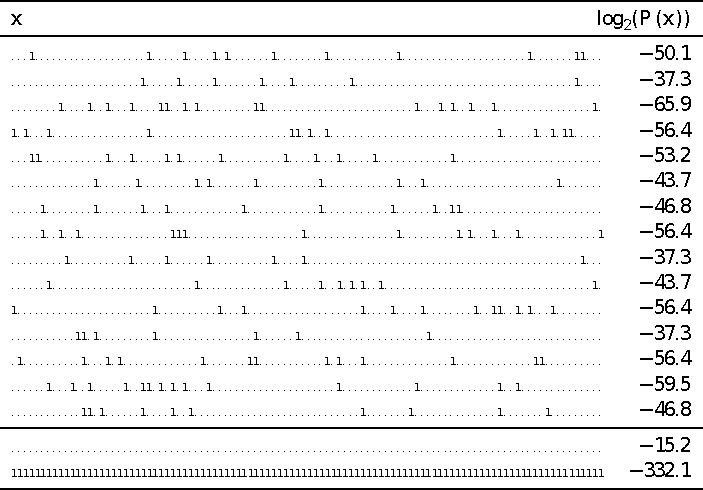
\includegraphics[width=0.5\textwidth]{images/seq100mackay.pdf}
  \caption{Sequências regadas por um ensaio de Bernoulli com $n=100$ e $P(X=1) = p = 0.1$. 
        As 15 sequências superiores representam amostras típicas. As duas últimas sequências
        representam a sequência mais provável e a menos provável \citep{mackay2003}.}
  \label{fig:seq100mackay}
  \end{figure}

  \framebreak

  \hvFloat[floatPos=htb,capPos=right,capVPos=bottom,objectPos=c]{figure}{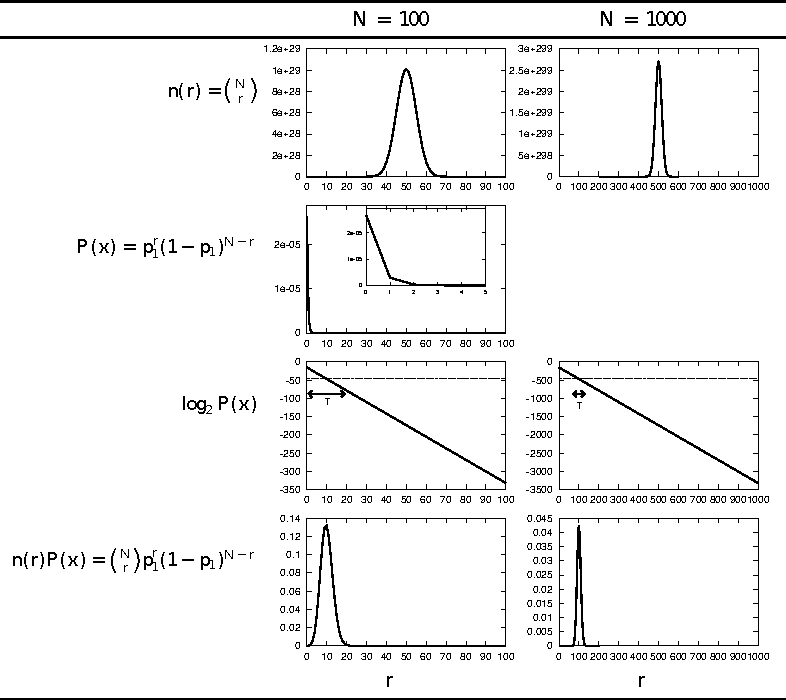
\includegraphics[width=0.5\textwidth]{images/seq100mackay2.pdf}}
  {Para $p=0.1$, $n=100$ e $n=1000$ os gráficos ilustram $n(r)$, o número de strings contendo
  $r$ 1s; a probabilidade $P(x_{1:n})$ para uma string contendo $r$ 1s; a mesma probabilidade
  em escala logarítmica; e a probabilidade total $n(r) P(x_{1:n})$ de todas as strings contendo $r$ 1s \citep{mackay2003}.}{fig:seq100mackay2}

  %\begin{figure}[h!]
  %\centering
  %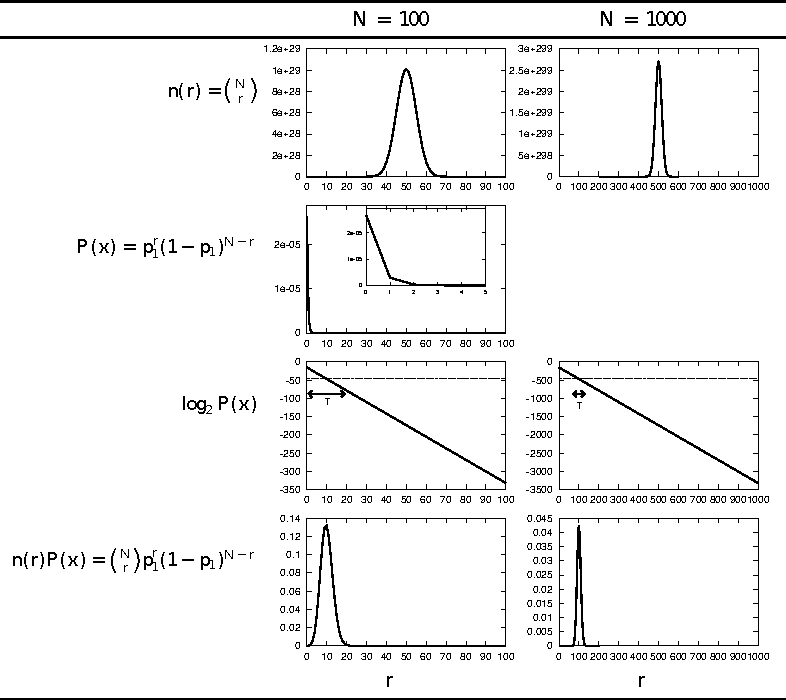
\includegraphics[width=0.5\textwidth]{images/seq100mackay2.pdf}
  %\caption{Para $p=0.1$, $n=100$ e $n=1000$ os gráficos ilustram $n(r)$, o número de strings contendo
  %      $r$ 1s; a probabilidade $P(x_{1:n})$ para uma string contendo $r$ 1s; a mesma probabilidade
  %      em escala logarítmica; e a probabilidade total $n(r) P(x_{1:n})$ de todas as strings contendo $r$ 1s \cite{mackay2003}.}
  %\label{fig:seq100mackay2}
  %\end{figure}


  \framebreak
  \begin{figure}[h!]
  \centering
  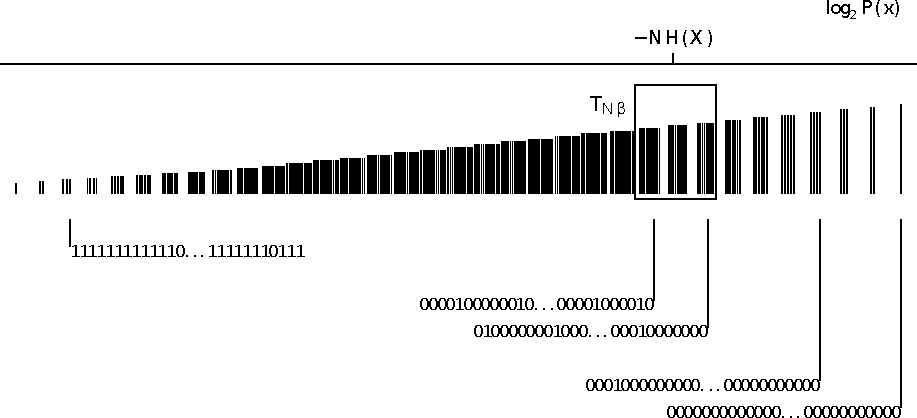
\includegraphics[width=0.5\textwidth]{images/seq100mackay3.pdf}
  \caption{Diagrama esquemático ilustrando todas as sequencias no conjunto $\mathcal{X}^n$ ordenadas pela probabilidade \citep{mackay2003}.}
  \label{fig:seq100mackay3}
  \end{figure}


  O termo \textbf{equipartição} é utilizado para descrever a ideia de que os membros do conjunto típico
  possuem aproximadamente a mesma probabilidade.

\end{frame}

\begin{frame}[allowframebreaks]
  \frametitle{Sequencias Típica - Exemplo: distribuição Binomial}
  $p(S_n = k) = {n \choose k} p^k q^{n-k}$, $S_n = X_1 + \ldots + X_n$, $X_i \sim \text{Bernoulli}(p)$
  Abaixo o gráfico dos valores normalizados $S_n/n = k/n$ para $p=0.5$.

  \hvFloat[floatPos=htb,capPos=right,capVPos=bottom,objectPos=c]{figure}{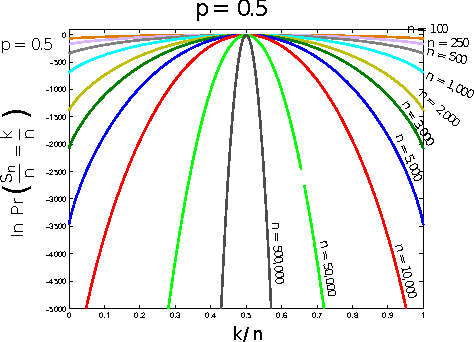
\includegraphics[width=0.5\textwidth]{images/bi-ex-ts.pdf}}
  {\citep{bilmes2013}.}{fig:bi-ex-ts}

  \framebreak

  $p(S_n = k) = {n \choose k} p^k q^{n-k}$, $S_n = X_1 + \ldots + X_n$, $X_i \sim \text{Bernoulli}(p)$
  Abaixo o gráfico dos valores normalizados $S_n/n = k/n$ para $p=0.9$.
  
   \hvFloat[floatPos=htb,capPos=right,capVPos=bottom,objectPos=c]{figure}{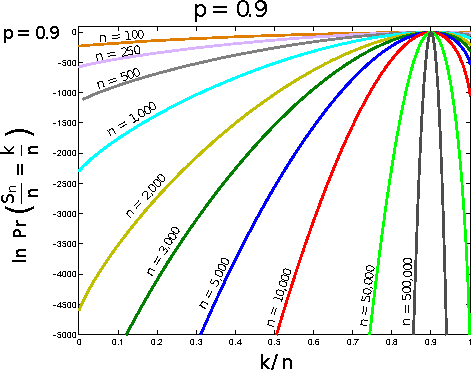
\includegraphics[width=0.5\textwidth]{images/bi-ex-ts9.pdf}}
  {\citep{bilmes2013}.}{fig:bi-ex-ts9}

\end{frame}
\note{
  Para comparação, o número de átomos no universo observável é $\approx e^{187} \approx 10^{81}$.

  \vspace{2cm}
  Uma imagem full HD ($1080 \times 720$ pixels) com 16 milhões de cores (24 bits por pixel) é representada por
  $K = 1080 \times 720 \times 24 = 18.662.400 \approx 10^{7}$ bits.
  Existem $2^K$ imagens possíveis, ou seja, $2^{18.662.400} \approx 10^{5.617 \times 10^6}$ sequências binárias 
  que representam imagens full HD com 16 milhões de cores, ou seja, um número \textbf{muito} maior do que o 
  número de átomos no universo. Obviamente, o conjunto de imagens que efetivamente ocorrem (ocorreram e ocorrerão
  ao longo de toda história da humanidade) é muito menos do que o número de possíveis imagens.
}


\begin{frame}%[allowframebreaks]
  \frametitle{Propriedades de $A_\epsilon^{(n)}$}
  \begin{theorem}[Propridades de $A_\epsilon^{(n)}$]
  \begin{enumerate}
  \item Se $(x_1, \ldots, x_n) \in A_\epsilon^{(n)}$, então
        \begin{equation}
        H(X) - \epsilon \leq - \frac{1}{n} \log p(x_1, \ldots, x_n) \leq H(X) + \epsilon
        \end{equation}
  \item $p(A_\epsilon^{(n)}) = p\left( \left\{ x: x \in A_\epsilon^{(n)} \right\} \right) > 1 - \epsilon$
        para $n$ grande suficiente, para todo $\epsilon > 0$.
  \item Limite superior: $\vert A_\epsilon^{(n)} \vert \leq 2^{n(H(X)+\epsilon)}$, onde
        $\vert A_\epsilon^{(n)} \vert$ é o número de elementos no conjunto $A_\epsilon^{(n)}$.
  \item Limite inferior: $\vert A_\epsilon^{(n)} \vert \geq (1-\epsilon) 2^{n(H(X)-\epsilon)}$ para
        $n$ grande suficiente.
  \end{enumerate}
  \end{theorem}
  
  \begin{itemize}
  \item O conjunto típico possui, essencialmente, probabilidade $1$ (algo típico irá tipicamente ocorrer).
  \item Todos os itens neste conjunto terão a mesma probabilidade $\approx 2^{-nH}$.
  \item O número de elementos neste conjunto é $\approx 2^{nH}$.
  \end{itemize}

\end{frame}


\begin{frame}%[allowframebreaks]
  \frametitle{Propriedades de $A_\epsilon^{(n)}$}
  \begin{proof}
  \begin{enumerate}
        \item O primeiro apenas é uma reformulação da definição de PEA.
        \item Vamos utilizar a definição expandida de convergência em probabilidade,
                dada na equação \ref{eq-pX1X2Xn-H}.
                \begin{equation}
                p(A_\epsilon^{(n)}) = p\left( \vert - \frac{1}{n} \sum_i \log p(x_i) - H \vert < \epsilon \right) > 1 - \delta 
                \end{equation}
                para $n$ grande suficiente. 
                Podemos escolher qualquer $\delta$, escolhemos então $\delta = \epsilon$, resultando em
                \begin{equation}
                p(A_\epsilon^{(n)}) > 1 - \epsilon, \quad \text{ para } n \text{ grande suficiente } \forall \epsilon
                \end{equation}
  \end{enumerate}
  \end{proof}
\end{frame}


\begin{frame}%[allowframebreaks]
  \frametitle{Propriedades de $A_\epsilon^{(n)}$}
  \begin{proof}
  \begin{enumerate}[3]
  \item Limite superior de $A_\epsilon^{(n)}$
        \begin{eqnarray}
        1 &=& \sum_x p(x) \geq \sum_{x \in A_\epsilon^{(n)}} p(x) \geq \sum_{x \in A_\epsilon^{(n)}} 2^{-n(H(X)+\epsilon)} \nonumber \\
        &=& \vert A_\epsilon^{(n)} \vert 2^{-n(H(X)+\epsilon)}
        \end{eqnarray}
        Resultando em $\vert A_\epsilon^{(n)} \vert \leq 2^{n(H+\epsilon)}$.
  \end{enumerate}
  \end{proof}
\end{frame}


\begin{frame}%[allowframebreaks]
  \frametitle{Propriedades de $A_\epsilon^{(n)}$}
  \begin{proof}
  \begin{enumerate}[4]
  \item Limite inferior do tamanho de $A_\epsilon^{(n)}$. Para $n$ grande suficiente
        \begin{eqnarray}
        1 - \epsilon &<& p(A_\epsilon^{(n)}) \leq \sum_{x \in A_\epsilon^{(n)}} 2^{-n(H(X)-\epsilon)} \nonumber \\
                &=& 2^{-n(H(X)-\epsilon)} \vert A_\epsilon^{(n)} \vert
        \end{eqnarray}
        resultando em $\vert A_\epsilon^{(n)} \vert \geq (1-\epsilon) 2^{n(H(X)-\epsilon)}$.
  \end{enumerate}
  \end{proof}
\end{frame}


\begin{frame}%[allowframebreaks]
  \frametitle{Codificação com Conjunto Típico}
  \begin{itemize}
  \item Existe um código que pode alcançar uma taxa de compressão de $H(X) + \epsilon'$ bits por
        símbolo para qualquer $\epsilon' > 0$ enquanto o comprimento do bloco $n$ 
        (o número de símbolos da fonte que são codificados simultâneamente) for grande suficiente.
  \item Mesmo que as mensagens da fonte sejam consideradas i.i.d., é necessário codificá-las
        conjuntamente de forma a alcançar esta taxa.
  \item Fazemos isso utilizando $n (H + \epsilon) + 2$ bits para cada sequencia típica, e
        utilizamos $n \log K + 2$ bits para cada sequência atípica. Este código é $1-1$ e 
        garantidamente livre de erros.
  \item De forma alternativa, podemos projetar para que exista um erro quando recebermos
        uma sequência atípica. Este código terá probabilidade de erro $P_e$.
  \item Em qualquer um dos casos, o comprimento esperado é
        \begin{equation}
        E[\frac{1}{n} l(X_{1:n})] \leq H(X) + \epsilon
        \end{equation}
  \item No segundo caso, $P_e \rightarrow 0$ quando $n \rightarrow \infty$.
  \end{itemize}
\end{frame}




\subsection{Compressão de Dados}

\begin{frame}%[allowframebreaks]
  \frametitle{Compressão de Dados até a Entropia da Fonte}
  Uma consequência importante é que podemos comprimir os dados até o limite da entropia da fonte.
  \begin{itemize}
  \item Ideia: considere $X_1, X_2, \ldots, X_n$ i.i.d. e $X_i \sim p(x)$.
  \item Particionar o conjunto de sequencias em dois blocos:
        \begin{itemize}
        \item Conjunto típico $A_\epsilon^{(n)}$
        \item e seu complemento, o conjunto não típico: $A_\epsilon^{(n)c} \triangleq \mathcal{X}^n \backslash A_\epsilon^{(n)}$.
        \end{itemize}
  \item Partições, i.e., $A_\epsilon^{(n)} \cap A_\epsilon^{(n)c} = \emptyset$ e $A_\epsilon^{(n)} \cup A_\epsilon^{(n)c} = \mathcal{X}^n$
  \end{itemize}

  \begin{figure}[h!]
  \centering
  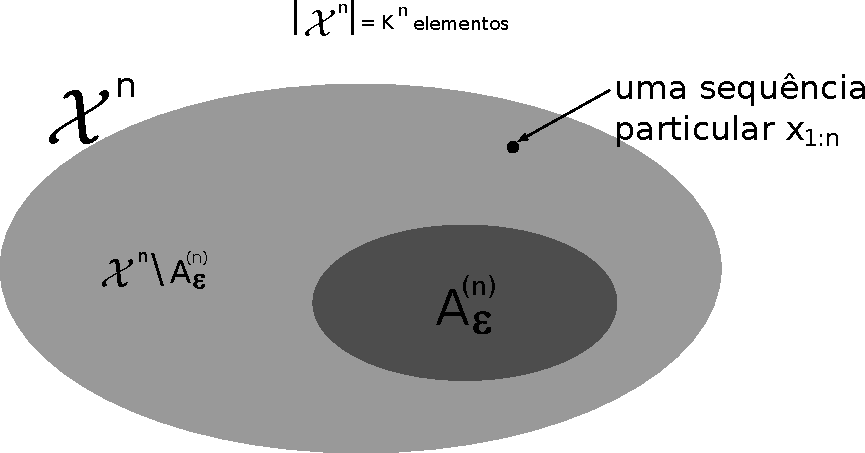
\includegraphics[width=0.5\textwidth]{images/particao2.pdf}
  %\caption{.}
  \label{fig:particao}
  \end{figure}

\end{frame}


\begin{frame}[allowframebreaks]
  \frametitle{Compressão do Conjunto Típico}
  \begin{itemize}
  \item Vamos indexar os elementos de cada conjunto (conjunto típico e não-típico) separadamente.
  \item O número de elementos do conjunto típico é $\vert A_\epsilon^{(n)} \vert \leq 2^{n(H+\epsilon)}$, 
        desta forma será necessário
        \begin{equation}
        \lceil n(H+\epsilon) \rceil \leq n (H + \epsilon) + 1 \text{ bits.}
        \end{equation}
  \item Podemos utilizar um bit extra para indicar se o elemento está no conjunto típico ou não, i.e.,
        vamos utilizar
        \begin{equation}
        (b_0,b_1,b_2,\ldots,b_{\lceil n(H+\epsilon) \rceil})
        \end{equation} 
        onde o primeiro bit indica se temos um elemento do conjunto típico ($b_0=0$) ou não 
        e os demais indexam o elemento do conjunto.
  \item O número total de bits necessário para uma sequência típica é $\leq n(H+\epsilon)+2$.
  \item Para os elementos do conjunto não típico, vamos utilizar 
        $\lceil \log \vert \mathcal{X} \vert^n \rceil \leq n \log K + 1$ bits.
  \item Vamos utilizar um vetor binário da forma
        \begin{equation}
        (b_0,b_1,b_2,\ldots,b_{\lceil \log \vert \mathcal{X} \vert^n \rceil})
        \end{equation}
        onde $b_0=1$, indicando a atipicidade.
  \item O número total de bits para uma sequência atípica é $\leq n \log K + 2$.
  \item Este código criado é 1-pra-1, sendo fácil codificar e decodificar, dado o \textit{codebook}
        (mapeamento).
  \item Para o conjunto não-típico $A_\epsilon^{(n)c}$ estamos utilizando mais bits do que o necessário,
        já que
        \begin{equation}
        \vert A_\epsilon^{(n)c} \vert = \vert \mathcal{X}^n \vert - \vert A_\epsilon^{(n)} \vert = 
        K^n - \vert A_\epsilon^{(n)} \vert \leq K^n ,
        \end{equation}
        mas isto não importará, como veremos adiante.
  \item As sequências típicas possuem um comprimento descritivo curto, $\approx nH$.
  \item Seja $l(x_{1:n})$ o comprimento da palavra (\textit{codeword}) associada à sequência $x_{1:n}$.
  \item $l(X_{1:n})$ é uma variável aleatória, já que $X_{1:n}$ é uma variável aleatória.
  \item Então $E l(X_{1:n}) = \sum_{x_{1:n}} p(x_{1:n}) l(x_{1:n})$ é o valor esperado do comprimento 
        do código. Queremos que ele seja o menor possível.
  \end{itemize}
\end{frame}


\begin{frame}[allowframebreaks]
  \frametitle{Comprimento Esperado}
  Suponha que $n$ seja grande suficiente de forma que $p(A_\epsilon^{(n)}) > 1 - \epsilon$, então
  \begin{eqnarray}
  E l(X_{1:n}) &=& \sum_{x_{1:n}} p(x_{1:n}) l(x_{1:n}) \nonumber \\
                &=& \sum_{x_{1:n} \in A_\epsilon^{(n)}} p(x_{1:n}) l(x_{1:n}) + \sum_{x_{1:n} \in A_\epsilon^{(n)c}} p(x_{1:n}) l(x_{1:n}) \nonumber \\
                &\leq& \sum_{x_{1:n} \in A_\epsilon^{(n)}} p(x_{1:n}) [n(H+\epsilon)+2] + \sum_{x_{1:n} \in A_\epsilon^{(n)c}} p(x_{1:n}) [n \log K + 2] \nonumber \\
                &=& \underbrace{p(A_\epsilon^{(n)})}_{\leq 1} [n(H+\epsilon)+2] + \underbrace{p(A_\epsilon^{(n)c})}_{< \epsilon} [n \log K + 2] \nonumber \\
                &\leq& n(H+\epsilon)+2 + \epsilon n \log K + \epsilon 2 \nonumber \\
                &=& n [H + \underbrace{\epsilon + \epsilon \log K + \frac{2}{n} + \frac{2 \epsilon}{n}}_{\epsilon'} ] = n(H+\epsilon')
  \end{eqnarray}

  \framebreak
  \begin{itemize}
  \item Podemos fazer $\epsilon'$ tão pequeno quanto queremos, fazendo $\epsilon$ pequeno e $n$ grande.
        \begin{equation}
        \epsilon' = \epsilon + \epsilon \log K + \frac{2}{n} + \frac{2 \epsilon}{n}
        \end{equation}
  \item Podemos então fazer $n(H+\epsilon')$ tão próximo quanto quisermos de $nH$, fazendo $\epsilon$ pequeno e $n$ grande.
  \end{itemize}
 
  \begin{theorem}[Primeiro Teorema de Shannon]
  Seja $X_{1:n}$ i.i.d. $\sim p(x)$, $\epsilon > 0$, então $\exists$ um código $f_n : \mathcal{X}^n \rightarrow \text{string binária}$
  e um inteiro $n_{\epsilon}$, tal que o mapeamento seja um-pra-um (desta forma inversível sem erro), e
        \begin{equation}
        E[ \frac{1}{n} l(X_{1:n})] \leq H(X) + \epsilon
        \end{equation}
  para todo $\epsilon > 0$ e todo $n \geq n_{\epsilon}$.
  \end{theorem}
  \begin{itemize}
  \item Será necessário no máximo $nH(X)$ bits para representar $X_{1:n}$, na média, ou $H(X)$ bits por símbolo do alfabeto da fonte.
  \item O primeiro teorema de Shannon diz que é possível (utilizando blocos de comprimento longo) comprimir até o limite da entropia.
  \item Exemplo: \textit{online coding} - codificar apenas o que é encontrado, sabendo que, para $n$ grande suficiente, aquilo que encontrar
        deve ser típico.
  \item É necessário ainda mostrar que não é possível comprimir abaixo do valor da entropia sem causar erros.
  \end{itemize}
\end{frame}

\begin{frame}[allowframebreaks]
  \frametitle{Existem outro conjunto muito provável?}
  \begin{itemize}
  \item Sabemos que $P(\mathcal{X}^n)=1$.
  \item Como $A_{\epsilon}^{(n)}$ é menor, teremos $P(A_{\epsilon}^{(n)}) \approx 1$.
  \item Existe um outro conjunto menor que contenha `toda' a probabilidade? Todos os elementos em $A_{\epsilon}^{(n)}$ 
        são essenciais? Se existir um conjunto menor, 
        podemos criar um código utilizando este conjunto e assim obter uma melhor compressão.
  \item Veremos que $A_{\epsilon}^{(n)}$ é o menor conjunto com `toda' a probabilidade.
  \end{itemize}

  \framebreak

  \begin{itemize}
  \item Vamos supor $B_{\delta}^{(n)}$ um conjunto qualquer com a propriedade
        \begin{equation}
        P(B_{\delta}^{(n)}) \geq 1 - \delta .
        \end{equation}
        $B_{\delta}^{(n)}$ contém as sequências mais prováveis.
  \end{itemize}

  \begin{theorem}
  Seja $X_{1:n}$ uma sequência i.i.d. $\sim p(x)$. Para $\delta < 1/2$ e qualquer $\delta' > 0$,
  se $P(B_{\delta}^{(n)}) > 1 - \delta$, então
        \begin{equation}
        \frac{1}{n} \log \vert B_{\delta}^{(n)} \vert >  H - \delta' \text{ se } n \text{ for grande suficiente}
        \end{equation}
        \begin{equation}
        \Rightarrow \vert B_{\delta}^{(n)} \vert > 2^{n(H-\delta')} \approx 2^{nH}
        \end{equation}
  \end{theorem}
  \begin{itemize}
  \item Assintoticamente $B_{\delta}^{(n)}$ não é menor do que $A_{\epsilon}^{(n)}$.
  \end{itemize}

  \framebreak

  \begin{definition}
  A notação $a_n \circeq b_n$ significa
        \begin{equation}
        \lim_{n \rightarrow \infty} \frac{1}{n} \log \frac{a_n}{b_n} = 0 ,
        \end{equation}
  então $a_n \circeq b_n$ implica que $a_n$ e $b_n$ são iguais até a primeira ordem do expoente.
  Ou seja, podemos dizer que para $n$ grande, $a_n$ e $b_n$ possuem aproximadamente o mesmo comportamento. 
  (Ver exemplos)
  \end{definition}
  Podemos então reescrever o teorema anterior da seguinte forma:
  \begin{theorem}
  Se $\delta_n \rightarrow 0$ e $\epsilon_n \rightarrow 0$, então teremos
        \begin{equation}
        \vert B_{\delta_n}^{(n)} \vert \circeq \vert A_{\epsilon_n}^{(n)} \vert \circeq 2^{nH}.
        \end{equation}
  \end{theorem}

  \framebreak

  \begin{proof}
  Seja $X_1, X_2, \ldots, X_n$ i.i.d. $\sim p(x)$. Seja $B_{\delta}^{(n)} \subset \mathcal{X}^n$ tal que
  $\Pr(B_{\delta}^{(n)}) > 1 - \delta$. Fixe $\epsilon < \frac{1}{2}$.
  Dados dois subconjuntos quaisquer $A$ e $B$ tais que $\Pr(A) > 1 - \epsilon_1$ e $\Pr(B) > 1 - \epsilon_2$.
  Seja $A^c$ o complemento de $A$ e $B^c$ o complemento de $B$, então
        \begin{equation}
        P(A^c \cup B^c) \leq P(A^c) + P(B^c) .
        \end{equation}

  \proofbreak

  Como $P(A) > 1 - \epsilon_1$, teremos $P(A^c) \leq \epsilon_1$. De forma similar, $P(B^c) \leq \epsilon_2$.
  Poderemos assim escrever
        \begin{eqnarray}
        P(A \cap B) &=& 1 - P(A^c \cup B^c) \nonumber \\
                &\geq& 1 - P(A^c) - P(B^c) \nonumber \\
                &\geq& 1 - \epsilon_1 - \epsilon_2.
        \end{eqnarray}

  Podemos reescrever a desigualdade anterior como
  \begin{equation}
  \Pr(A_{\epsilon}^{(n)} \cap B_{\delta}^{(n)}) \geq 1 - \epsilon - \delta .
  \end{equation}

  \proofbreak

  A probabilidade de um conjunto é dada pela soma das probabilidades de todos os elementos (sequências) neste conjunto, logo teremos
  \begin{equation}
  \Pr(A_{\epsilon}^{(n)} \cap B_{\delta}^{(n)}) = \sum_{x^n \in A_{\epsilon}^{(n)} \cap B_{\delta}^{(n)}} p(x^n)
  \end{equation}
  A probabilidade dos elementos no conjunto típico é limitada por $2^{-n(H-\epsilon)}$. 

  \proofbreak
  Desta forma teremos
  \begin{eqnarray}
  1 - \epsilon - \delta &\leq& \Pr(A_{\epsilon}^{(n)} \cap B_{\delta}^{(n)}) \nonumber \\
                &=& \sum_{x^n \in A_{\epsilon}^{(n)} \cap B_{\delta}^{(n)}} p(x^n) \nonumber \\
                &\leq& \sum_{x^n \in A_{\epsilon}^{(n)} \cap B_{\delta}^{(n)}} 2^{-n(H-\epsilon)} \nonumber \\
                &=& \vert A_{\epsilon}^{(n)} \cap B_{\delta}^{(n)} \vert 2^{-n(H-\epsilon)} \nonumber \\
                &\leq& \vert B_{\delta}^{(n)} \vert 2^{-n(H-\epsilon)},
  \end{eqnarray} 
  onde utilizamos $A_{\epsilon}^{(n)} \cap B_{\delta}^{(n)} \subseteq B_{\delta}^{(n)}$.

  \proofbreak
  Poderemos reescrever então da seguinte forma,
  \begin{equation}
  \vert B_{\delta}^{(n)} \vert  >  2^{n(H-\epsilon)} ,
  \end{equation}
  onde $\epsilon > 0$.

  \end{proof}

  \framebreak

  Vejamos alguns exemplos para entender o significado de $a_n \circeq b_n$.
  \begin{example}
  Suponha que a sequência $a_n$ seja definida como $a_n = e^{3n+1}$ e a $b_n$ definida como $b_n = e^{3n}$.
  Teremos que
  \begin{equation}
   \log \frac{a_n}{b_n} = \log e ,
  \end{equation}
  ou seja, embora $a_n$ e $b_n$ sejam diferentes em todos os pontos, sendo $a_n$ maior que $b_n$ por 
  um fator constante $e$, o logarítmo da razão entre ambas sequências não cresce muito rápido, o que pode ser
  verificado por
  \begin{equation}
   \lim_{n \rightarrow \infty} \frac{1}{n} \log \frac{a_n}{b_n} = \lim_{n \rightarrow \infty} \frac{\log e}{n} = 0 .
  \end{equation}
  \end{example}

  \framebreak

  \begin{example}
  Considere agora $a_n = e^{3n + \sqrt{n}}$ e $b_n = e^{3n}$. Então 
  \begin{equation}
   \lim_{n \rightarrow \infty} \frac{1}{n} \log \frac{a_n}{b_n} = \lim_{n \rightarrow \infty} \frac{1}{n} \sqrt{n} = \lim_{n \rightarrow \infty} \frac{1}{\sqrt{n}} = 0 .
  \end{equation}
  Embora agora a razão entre $a_n$ e $b_n$ seja crescente com $n$, seu crescimento é lento.
  \end{example} 

  \framebreak

  \begin{example}
  Seja $a_n = e^{4n}$ e $b_n = e^{3n}$. Teremos agora
  \begin{equation}
   \lim_{n \rightarrow \infty} \frac{1}{n} \log \frac{a_n}{b_n} = \lim_{n \rightarrow \infty} \frac{1}{n} n = 1 .
  \end{equation}  
  Neste caso, a razão entre $a_n$ e $b_n$ cresce muito rápido, o que foi constatado ao verificar que o limite 
  da razão acima não convergiu para zero.  
  \end{example}

\end{frame}



\begin{frame}[allowframebreaks]
  \frametitle{Estratégia de codificação com erros}
  \begin{itemize}
  \item Considere uma variação do código anterior que pode cometer erros.
  \item Sequências típicas utilizarão $nH$ bits.
  \item Sequências atípicas serão mapeadas arbitrariamente em palavras curtas.
  \end{itemize}

  \begin{figure}[h!]
  \centering
  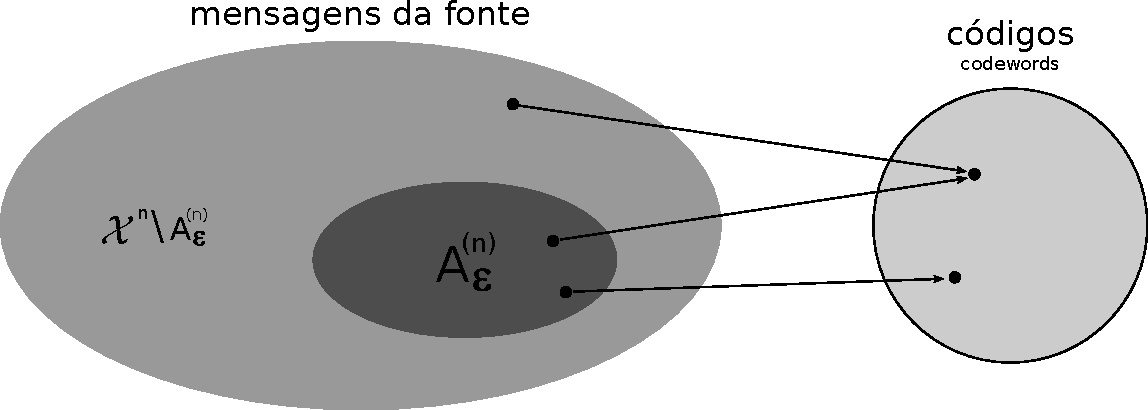
\includegraphics[width=0.75\textwidth]{images/code-with-error2.pdf}
  %\caption{.}
  \label{fig:code-with-error}
  \end{figure}

  \framebreak

  \begin{itemize}
  \item Sabemos que $P(A_{\epsilon}^{(n)}) > 1 - \epsilon$.
  \item Um erro ocorre quando a sequência não é típica, logo a probabilidade de erro $P_e$ é limitada por
        \begin{equation}
        P_e = P(A_{\epsilon}^{(n)c}) \leq \epsilon
        \end{equation}
  \item Conjunto típico: $\forall \epsilon > 0$, $\forall \delta > 0$, $\exists n_0$ tal que, para $n > n_0$,
        \begin{equation}
        p \left\{ \vert - \frac{1}{n} \log p(x_1, \ldots, x_n) - H \vert > \epsilon \right\} \leq \delta
        \end{equation}
        Podemos pensar como se fosse uma função $\delta(n,\epsilon)$ com $\lim_{n \rightarrow \infty} \delta(n,\epsilon) = 0$ para todo $\epsilon > 0$.
  \item Teremos então $P_e = P(A_{\epsilon}^{(n)c}) \leq \delta(n,\epsilon)$ 
        \begin{equation}
        P_e \rightarrow 0 \text{ à medida que } n \rightarrow \infty
        \end{equation}
  \item Independente de utilizarmos uma palavra longa e não tivermos erro, ou tivemos erro, 
        o comprimento esperado é o mesmo e a probabilidade de erro vai pra zero se codificarmos o conjunto típico.
  \end{itemize}

\end{frame}


\begin{frame}[allowframebreaks]
  \frametitle{Codificando com menos do que $H$ bits}
  \begin{itemize}
  \item O primeiro teorema de Shannon afirma que a codificação será sem erro se utilizarmos $n(H+\epsilon)$ bits 
        por palavra código, para qualquer $\epsilon > 0$. O que ocorre se utilizarmos menos?
  \item Se utilizarmos $n(H-\alpha \epsilon)$ bits por palavra, com $\alpha > 1$, teremos no máximo $2^{n(H-\alpha \epsilon)}$ palavras.
  \item $2^{-n(H-\epsilon)}$ é o limite superior da probabilidade de sequências típicas.
  \item A probabilidade de sequências para as quais seremos capazes de fornecer uma palavra código não será maior do que o produto
        \begin{equation}
        2^{n(H-\alpha \epsilon)} 2^{-n(H-\epsilon)} = 2^{-n\epsilon(\alpha - 1)}
        \end{equation}
  \item Para qualquer $\alpha > 1$, esta probabilidade $\rightarrow 0$ quando $n \rightarrow \infty$.
  \item Problema: a probabilidade de sermos capazes de fornecer palavras código irá diminuir exponencialmente com $n$, pois a 
        probabilidade da tipicidade diminui exponencialmente mais rápido do que o crescimento do número de códigos com $n$.
  \item O erro vai para $1$ quando $n \rightarrow \infty$.
  \item Dadas $n$ v.a.s com entropia $H$, podemos comprimi-las com mais do que $nH$ bits com um risco mínimo de perder informação, quando $n \rightarrow \infty$.
        De maneira oposta, se as v.a.s são comprimidas a menos do que $nH$ bits, então é virtualmente certo que haverá perda de informação e incorremos em erro.
  \end{itemize}

\end{frame}

\begin{frame}[allowframebreaks]
  \frametitle{Codificação do conjunto típico / Compressão (resumo)}
  \begin{itemize}
  \item Existe um código que pode alcançar uma taxa de compressão de $H(X) + \epsilon'$ bits por símbolo da fonte, para
        qualquer $\epsilon'>0$, enquanto o comprimento do bloco $n$ (número de símbolos da fonte que são codificados simultaneamente) for longo suficiente.
  \item Embora as sequências produzidas pelas fonte são consideradas i.i.d., é necessário codificá-las conjuntamente para atingir esta taxa.
  \item Fazemos isto utilizando $n(H+\epsilon)+2$ bits para cada sequência típica e $n \log K + 2$ bits para cada sequência atípica. Este código
        é 1-1 e garantidamente sem erro.
  \item De maneira alternativa, podemos projetar para que ocorra um erro quando recebermos uma sequência atípica. O código possui uma
        probabilidade de erro $P_e$ que não será nula, mas $\rightarrow 0$ exponencialmente rápido, quando $n \rightarrow \infty$, se $\epsilon'>0$.
  \item Em qualquer caso, o comprimento esperado é
        \begin{equation}
        E[\frac{1}{n} l (X_{1:n})] \leq H(X) + \epsilon
        \end{equation}
  \end{itemize}
\end{frame}


